\documentclass[11pt]{book}
%\usepackage[subpreambles=true]{standalone}
\usepackage[spanish]{babel}
\usepackage{comfortaa}
\usepackage[T1]{fontenc}
\usepackage[utf8]{inputenc}
\usepackage[
letterpaper,
left=1in, 
right=1in, 
top=1in,
bottom=1in,
headheight=10mm,% Set \headheight to 10mm
]{geometry} % Custom margins
\usepackage{float}
\usepackage[colorlinks = true, linkcolor = colorrds]{hyperref}
\usepackage{bookmark}
\usepackage{fancyhdr}
\usepackage{color, colortbl}
\usepackage[dvipsnames,table]{xcolor} % Required for custom color
\usepackage{graphicx}
\usepackage{tabularx}
\usepackage{multicol,multirow}
\usepackage{newclude}
\usepackage{tabto}
\usepackage{remreset}
\usepackage[inline]{enumitem}
\usepackage{xparse}
\usepackage{wrapfig}
\usepackage{caption,capt-of}
\usepackage{amssymb,amsmath}
\usepackage{tikz}
\usepackage{etoolbox}
\usepackage{pdflscape}
\usepackage[explicit]{titlesec}
\usepackage{subfiles} % Best loaded last in the preamble
\input{insbox}
\makeatletter
\@removefromreset{section}{chapter}
\makeatother
\addto\captionsspanish{\renewcommand{\chaptername}{Unidad}}
\renewcommand{\thechapter}{\arabic{chapter}}
\renewcommand{\thesection}{S\arabic{section}}
\renewcommand{\thesubsection}{L\arabic{subsection}}
\newcommand*\chapterlabel{}
\titleformat{\chapter}
{\gdef\chapterlabel{}
    \comfortaa\Huge\bfseries
}
{\gdef\chapterlabel{\chaptername \ \thechapter}}{0pt}
{\begin{tikzpicture}[remember picture,overlay]
        \node[yshift=-2cm] at (current page.north west)
        {\begin{tikzpicture}[remember picture, overlay]
                \draw[draw=none,fill=teal] (0,0) rectangle
                (\paperwidth,2cm);
                \node[anchor=east,xshift=.9\paperwidth,rectangle,
                    rounded corners=5pt,inner xsep=20pt,inner ysep=5pt,
                    blur shadow={shadow blur steps=50,shadow blur extra rounding=5pt},
                    fill=brown]
                {\color{CadetBlue!20}\textbf{\chapterlabel#1}};
            \end{tikzpicture}
        };
    \end{tikzpicture}
}
\titlespacing*{\chapter}{0pt}{50pt}{-60pt}

\makeatletter
\@removefromreset{section}{chapter}
\makeatother
\addto\captionsspanish{\renewcommand{\chaptername}{Unidad}}
\renewcommand{\thechapter}{\arabic{chapter}}
\renewcommand{\thesection}{S\arabic{section}}
\renewcommand{\thesubsection}{L\arabic{subsection}}
\newcommand*\sectionlabel{}
\titleformat{\section}
{\gdef\sectionlabel{}
    \comfortaa\large\bfseries
}
{\gdef\sectionlabel{\thesection \ }}{0pt}
{\begin{tikzpicture}[remember picture,overlay]
        \node[yshift=-1.5cm] at (current page.north west)
        {\begin{tikzpicture}[remember picture, overlay]
                \draw[draw=none,fill=colorrds!30,
                    %shade,
                    rounded corners=5pt,
                    blur shadow={shadow blur steps=10,shadow blur extra rounding=10pt},
                    xshift=5mm,
                ] (0,0) rectangle
                (\paperwidth-10mm,2cm);
                \node[
                    anchor=west,
                    xshift=0.1\paperwidth,
                    rectangle,
                    %shade,
                    rounded corners=5pt,
                    inner sep=8pt,
                    fill=olive!50,
                    %drop shadow={fill=black, opacity=1},
                ]
                {\color{colorrds}\sectionlabel#1};
                % \node[anchor=east,xshift=.9\paperwidth,rectangle,
                %     rounded corners=10pt,inner sep=11pt,
                %     fill=blue!35]
                % {\color{green}\sectionlabel};
            \end{tikzpicture}
        };
    \end{tikzpicture}
}
\titlespacing*{\section}{0pt}{50pt}{0pt}
\usepackage[many]{tcolorbox}
% \usepackage{mathspec} 			    % for FONTS
% \usepackage{setspace}               % for LINE SPACING
% \setmainfont{Noto Sans}[
%     Kerning = On,
%     Mapping = tex-text,
%     Numbers = Uppercase,
%     BoldFont = Noto Sans SemiBold
% ]                           % setting the font as Noto Sans
% \setlength\parindent{0pt}   % killing indentation for all the text
% \setstretch{1.3}            % setting line spacing to 1.3
% \setlength\columnsep{0.25in} % setting length of column separator
% \pagestyle{empty}           % setting pagestyle to be empty


\definecolor{main}{HTML}{5989cf}    % setting main color to be used
\definecolor{sub}{HTML}{cde4ff}     % setting sub color to be used

\tcbset{
    sharp corners,
    colback = white,
    before skip = 0.2cm,    % add extra space before the box
    after skip = 0.5cm      % add extra space after the box
}                           % setting global options for tcolorbox


\newtcolorbox{bA}{
    %sharpish corners, % b
    enhanced,
    %colback = sub, % background color
    boxrule = 0.2pt,  % no borders
    %borderline = {1pt}{1pt}{black!35}, % add "dashed" for dashed line
    %fontupper = \bf\color{black}, % font color
    %colframe = main % frame color
    rounded corners,
    %arc = 5pt,   % corners roundness
    fuzzy shadow = {2pt}{-4pt}{-1pt}{1pt}{black!35}, % {xshift}{yshift}{offset}{step}{options} 
    %toprule = 3pt, % top rule weight
    %bottomrule = 3pt % bottom rule weight
}
% You can copy any following box you like to your code.
\newtcolorbox{boxA}{
    fontupper = \bf,
    boxrule = 1.5pt,
    colframe = black % frame color
}

\newtcolorbox{boxB}{
    fontupper = \bf\color{main}, % font color
    boxrule = 1.5pt,
    colframe = main,
    rounded corners,
    arc = 5pt   % corners roundness
}

\newtcolorbox{boxC}{
    colback = sub, % background color
    boxrule = 0pt  % no borders
}

\newtcolorbox{boxD}{
    colback = sub,
    colframe = main,
    boxrule = 0pt,
    toprule = 3pt, % top rule weight
    bottomrule = 3pt % bottom rule weight
}

\newtcolorbox{boxE}{
    enhanced, % for a fancier setting,
    boxrule = 0pt, % clearing the default rule
    borderline = {0.75pt}{0pt}{main}, % outer line
    borderline = {0.75pt}{2pt}{sub} % inner line
}

\newtcolorbox{boxF}{
    colback = sub,
    enhanced,
    boxrule = 1.5pt,
    colframe = white, % making the base for dash line
    borderline = {1.5pt}{0pt}{main, dashed} % add "dashed" for dashed line
}

\newtcolorbox{boxG}{
    enhanced,
    boxrule = 0pt,
    colback = sub,
    borderline west = {1pt}{0pt}{main},
    borderline west = {0.75pt}{2pt}{main},
    borderline east = {1pt}{0pt}{main},
    borderline east = {0.75pt}{2pt}{main}
}

\newtcolorbox{boxH}{
    colback = colorrds!10,
    colframe = colorrds,
    boxrule = 0pt,
    leftrule = 6pt % left rule weight
}

\newtcolorbox{boxI}{
    colback = sub,
    colframe = main,
    boxrule = 0pt,
    toprule = 6pt % top rule weight
}

\newtcolorbox{boxJ}{
    sharpish corners, % better drop shadow
    colback = sub,
    colframe = main,
    boxrule = 0pt,
    toprule = 4.5pt, % top rule weight
    enhanced,
    fuzzy shadow = {0pt}{-2pt}{-0.5pt}{0.5pt}{black!35} % {xshift}{yshift}{offset}{step}{options} 
}

\newtcolorbox{boxK}{
    sharpish corners, % better drop shadow
    boxrule = 0pt,
    toprule = 4.5pt, % top rule weight
    enhanced,
    fuzzy shadow = {0pt}{-4pt}{-1pt}{1pt}{black!35} % {xshift}{yshift}{offset}{step}{options} 
}

\newtcolorbox{boxL}{
    fontupper = \color{main},
    rounded corners,
    arc = 6pt,
    colback = sub,
    colframe = main!50,
    boxrule = 0pt,
    bottomrule = 4.5pt
}

\newtcolorbox{boxM}{
    fontupper = \color{white},
    rounded corners,
    arc = 6pt,
    colback = main!80,
    colframe = main,
    boxrule = 0pt,
    bottomrule = 4.5pt,
    enhanced,
    fuzzy shadow = {0pt}{-3pt}{-0.5pt}{0.5pt}{black!35}
}
\decimalpoint
%\captionsetup{width=.45\textwidth}
\setlength{\parindent}{0pt}
\graphicspath{{./Images}} %Setting the graphicspath
\definecolor{colorrds}{HTML}{0060A0} % Custom colour
%%% Headings and footer
\renewcommand\spanishtablename{Tabla}
\cfoot{\thepage}
\renewcommand{\headrulewidth}{0.2pt}
\renewcommand{\footrulewidth}{0.2pt}
%%%
\usetikzlibrary{
  arrows,
  positioning,
  matrix,
  calc,
  decorations.pathreplacing,
  decorations.pathmorphing,
  decorations.markings,
  decorations.text,
  shapes.symbols,
  backgrounds,
  shadows.blur,
  trees,
  fit,
  snakes,
  patterns,
  mindmap,
  intersections,
  calendar,
  plotmarks,
  spy,
  tikzmark}

%%%% APRENDISAJES TEXTBOX
\tikzset{
  abstractbox/.style={
    draw=black, fill=white, rectangle, 
    inner sep=15pt, style=rounded corners,
    drop shadow={fill=black, opacity=1}
  },
  abstracttitle/.style={fill=white}
}
\newcommand{\boxabstract}[2][fill=white]{
  \begin{tikzpicture}
    \node [abstractbox, #1] (box)
    {\begin{minipage}{0.9\linewidth}
        \setlength{\parindent}{0mm} % Indentar.
        \normalfont #2
      \end{minipage}};
    \node[abstracttitle, right=5pt] at (box.north west) {\textbf{Aprendizajes esperados:}};
    \node[draw=none, fit=(box)] {};
  \end{tikzpicture}
}%
%%%%%%%%%%%%%%%%%%%%%%%%
%\renewcommand{\labelenumi}{\mbox{\arabic{enumi}}}
%\%renewcommand{\labelitemi}{$\square$}

%%%%%%%%%%%%% START questions env
%Idea from https://tex.stackexchange.com/a/236668/1952
% \DeclareDocumentCommand\question{o}{%
%     \item\IfNoValueTF{#1}{}{(#1 puntos)}}
% \newenvironment{questions}[1][]{\enumerate[,#1]}{\endenumerate}
%\DeclareDocumentCommand\part{o}{%
% \item\IfNoValueTF{#1}{}{(#1 puntos)}}
% \newenvironment{parts}[1][]{\enumerate[,#1]}{\endenumerate}
% \newcommand{\part}{\item}
%%\newcommand{\choice}{\item}
% \newlist{parts}{enumerate*}{1}
% \setlist[parts,1]{label=(\alph*), itemjoin={{\quad}},leftmargin = 1cm}
% \newlist{oneparchoices}{enumerate*}{1}
% \setlist[oneparchoices,1]{label=\quad\alph*), itemjoin={{\quad}},leftmargin = 1cm}
% \newlist{choices}{itemize}{1}
% \setlist[choices,1]{label=\quad$\square$, itemjoin={{\\}},leftmargin = 1cm}
\newlist{hoptboxes}{itemize*}{1}
\setlist[hoptboxes,1]{label=\Large$\square$, font=\color{colorrds},itemjoin={{\quad}},leftmargin = 1cm}
\newlist{hoptions}{enumerate*}{1}
\setlist[hoptions,1]{label=(\alph*), font=\color{colorrds},itemjoin={{\quad}},leftmargin = 1cm}
%%%%%%%%%%%%% END questions env
\newenvironment{mybox}[3][]{%
  \begin{tikzpicture}[#1]%
    \def\myboxname{#3}%
    % good options: minimum height, minimum width
    \node [draw, inner sep=2ex,  align=justify]
      (BOXCONTENT) \bgroup\rule{0ex}{0ex}\ignorespaces
  }{%
    \egroup;
    \node [right, inner sep=3pt, fill=colorrds!75, outer sep=0pt, 
      text height=2ex, text depth=.5ex] (BOXNAME) 
      at ([shift={(-1em,5pt)}]BOXCONTENT.north west) {\myboxname};
    \fill[colorrds] (BOXNAME.north east) -- +(-1em,1em)
      -- +(-1em,0) -- cycle;
    \fill[colorrds] (BOXNAME.south west) -- +(1em,-1em)
      -- +(1em,0) -- cycle;
  \end{tikzpicture}
}
\begin{document}
\pagestyle{empty}
\newgeometry{left=0mm,top=50mm,bottom=0mm,right=0mm}
\documentclass[]{book}
\usepackage{geometry,graphicx} % Custom margins
\usepackage[spanish]{babel}
\usepackage[T1]{fontenc}
\usepackage[dvipsnames]{xcolor} % Required for custom color
\usepackage{color,colortbl}
\usepackage[utf8]{inputenc}
\usepackage{geometry} % Custom margins
\usepackage[spanish]{babel}
\usepackage{adjustbox,dashbox}
\usepackage{array}
\usepackage{tikz,pgfplots,pgfkeys}
\usepackage{forest,mathtools,siunitx}
\usepackage{amsfonts, amssymb, amsxtra, amsmath, amsbsy}
\usepackage{newclude}
\usepackage{ifthen}
\usepackage{float}
\usepackage{fancybox}
\usepackage{graphicx,tabularx}
\usepackage{multicol,multirow}
\usepackage{enumitem} % Customising the numbered lists
\usepackage{xhfill} % Making the pink block not extend beyond the margin
\usepackage{nameref} % reference the names of the sections
\usepackage{caption,capt-of}
\usepackage[normalem]{ulem} % Dashed lines in appendix
\usepackage{ragged2e} % Ragged left
\usepackage{booktabs}
\usepackage[unboxed]{cwpuzzle}
\usepackage[colorlinks = true,linkcolor = blue]{hyperref}
\usepackage{subfiles}
\usepackage{wrapfig}
\input{insbox}
\usepackage{etoolbox}
\usepackage{mwe}
\usepackage{comfortaa}
\usepackage[T1]{fontenc}
\renewcommand*\oldstylenums[1]{{\firaoldstyle #1}}
\usepackage[T1]{fontenc}
\usepackage{pythontex}
\usepackage{polynom}
\usepackage{longdivision}


\title{Actividades}
\author{Julio C. Melchor P.\thanks{{\tt julio.melchor@rafaeldiazserdan.net}}}
\date{v1.0, \today}
%\usepackage[dvipsnames]{xcolor} % Required for custom color
\usepackage{color,colortbl}
\usepackage[utf8]{inputenc}
\usepackage{geometry} % Custom margins
\usepackage[spanish]{babel}
\usepackage{adjustbox,dashbox}
\usepackage{array}
\usepackage{tikz,pgfplots,pgfkeys}
\usepackage{forest,mathtools,siunitx}
\usepackage{amsfonts, amssymb, amsxtra, amsmath, amsbsy}
\usepackage{newclude}
\usepackage{ifthen}
\usepackage{float}
\usepackage{fancybox}
\usepackage{graphicx,tabularx}
\usepackage{multicol,multirow}
\usepackage{enumitem} % Customising the numbered lists
\usepackage{xhfill} % Making the pink block not extend beyond the margin
\usepackage{nameref} % reference the names of the sections
\usepackage{caption,capt-of}
\usepackage[normalem]{ulem} % Dashed lines in appendix
\usepackage{ragged2e} % Ragged left
\usepackage{booktabs}
\usepackage[unboxed]{cwpuzzle}
\usepackage[colorlinks = true,linkcolor = blue]{hyperref}
\usepackage{subfiles}
\usepackage{wrapfig}
\input{insbox}
\usepackage{etoolbox}
\usepackage{mwe}
\usepackage{comfortaa}
\usepackage[T1]{fontenc}
\renewcommand*\oldstylenums[1]{{\firaoldstyle #1}}
\usepackage[T1]{fontenc}
\usepackage{pythontex}
\usepackage{polynom}
\usepackage{longdivision}

 % Imports all the required packages. See Functional/%Packages.tex for more detailS
\geometry{letterpaper,total={175mm,220mm},left=15mm,top=50mm,bottom=0mm} % Custom margins

\begin{document}
\pagestyle{empty}
\begin{center}
    {\Huge Matem\'aticas 3}\\
    \vspace{1cm}
    \normalsize
    \textbf{\large Cuaderno de trabajo}\\
    para los alumnos de 3$^\circ$ de  Secundaria\\
    en el curso durante el ciclo escolar\\
    \textbf{2022-2023}\\
    \vspace{2.2cm}
    \small POR\\
    \Large J. C. Melchor Pinto\\[0.5em]
    \normalsize Profesor de asignatura en\\
    \vspace{1cm}
    
\includegraphics[width=5cm]{../Unidad 2/Images/LOGO_RDS_nobg}
\end{center}
\vspace{2.5cm}
%\include*{Functional/TitlePage}
\hspace{-16mm}
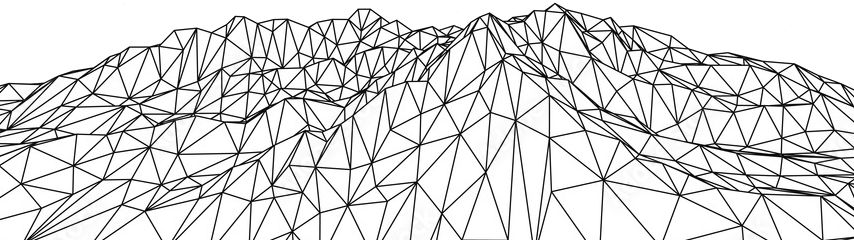
\includegraphics[width=\paperwidth]{../Unidad 2/Images/cover_bg}
\end{document}

\restoregeometry
\addtocontents{toc}{\setcounter{tocdepth}{3}}
\tableofcontents
\newpage
\chapter{}
\pagestyle{fancy}
\newpage \thispagestyle{plain}
\section{Múltiplos y divisores}
\subsection{Múltiplos}
\subsection{Divisores}
\subsection{Problemas de multiplicación y división de fracciones}
\subsection{Multiplicación de números positivos y negativos}

\newpage \thispagestyle{plain}
\section{Números primos}
\subsection{Números primos y compuestos}
\subsection{Factorización y descomposición en números primos}

\newpage \thispagestyle{plain}
\section{Mínimo común múltiplo y máximo común divisor}
\subsection{Mínimo común múltiplo}
\subsection{Máximo común divisor}

\newpage \thispagestyle{plain}
\section{Polígonos semejantes}
\subsection{Semejanza de polígonos}
\subsection{Construcción de polígonos semejantes}

\newpage \thispagestyle{plain}
\section{Criterios de semejanza de triángulos}
\subsection{Criterios de semejanza de triángulos}
\subsection{Aplicaciones de semejanza de triángulos}

\newpage \thispagestyle{plain}
\section{Medidas de tendencia central y de dispersión}
\subsection{Significado de las medidas de tendencia central}
\subsection{Significado de las medidas de dispersión}
\subsection{Comparación de dos conjuntos de datos}

\newpage
\chapter{}

\newpage \thispagestyle{plain}
\section{Ecuaciones cuadráticas}
\boxabstract{Resuelve problemas mediante la formulación y la solución algebraica de ecuaciones cuadráticas.}
\subsection{Ecuaciones cuadráticas}

Analiza las situaciones y contesta lo que se pide.\\

\begin{boxK}
    \begin{center}\textbf{Inicio}\end{center}
    Lee la situación, observa la imagen y responde lo que se pide.
    \begin{enumerate}
        \item Martín fue contratado para cercar un terreno con 120 m de malla. Le pidió a su cliente
              los datos del terreno, quien se los entregó en un papel. Al llegar a su casa, Martín se dio
              cuenta de que perdió la información y sólo recordó que el triple del ancho menos el
              largo es igual a 28 m. No quiso llamar nuevamente al cliente y determinó las dimensio-
              nes del terreno. \textbf{¿Cuáles son?}
              \begin{enumerate}
                  \item Asigna variables y escribe las ecuaciones que modelan la situación.
                  \item Describe un procedimiento para resolverlas.
                  \item Determina las medidas de los lados del terreno.
                  \item ¿Qué información es relevante para responder y
                        cuál no?
                  \item Describe tu procedimiento para saber las respuestas.
              \end{enumerate}
    \end{enumerate}

\end{boxK}

\begin{enumerate}
    \item El hotel \emph{El Sol} gestionó con el municipio tener una zona de nado en el mar
          para el disfrute de sus huéspedes. Le han asignado 600 m$^2$ de superficie
          de mar y debe delimitarla con una cuerda y boyas para seguridad de los
          bañistas. El gerente del hotel quiere que la zona sea cuadrada, \\
          \textbf{¿cuál es la longitud de los lados? (figura \ref{fig:square})}.

          \begin{minipage}{.45\textwidth}
              \begin{figure}[H]
                  \centering
                  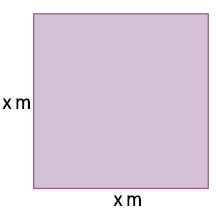
\includegraphics[width=0.4\linewidth]{square.png}
                  \captionof{figure}{Modelo geométrico de la situación.}
                  \label{fig:square}
              \end{figure}%
          \end{minipage}\hfill
          \begin{minipage}{.45\textwidth}
              \begin{figure}[H]
                  \centering
                  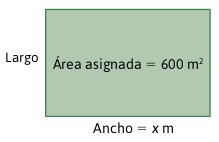
\includegraphics[width=0.6\linewidth]{square2.png}
                  \captionof{figure}{Modelo geométrico de la situación.}
                  \label{fig:square2}
              \end{figure}
          \end{minipage}

          \begin{enumerate}
              \item ¿Cuáles son las cantidades conocidas?
              \item ¿Cuáles son las cantidades desconocidas?
              \item Escriban una ecuación que modele la situación.
              \item ¿Cuál es la longitud de los lados?
          \end{enumerate}

    \item Antes de que se hiciera la delimitación de la zona de nado, el gerente del
          hotel cambió de opinión acerca de la forma de esta zona. Ahora debía
          ser rectangular con cierta característica: el largo tiene 10 m menos que
          el ancho. \textbf{¿Cuál es la longitud de los lados de la superficie delimitada?
              (figura \ref{fig:square2})}.\\
          \begin{enumerate}
              \item ¿Cuáles son las cantidades conocidas?
              \item ¿Cuáles son las cantidades desconocidas?
              \item Escriban una ecuación que modele la situación.
              \item Planteen una forma de resolver el problema. ¿Cuál es la longitud de los
                    lados?
          \end{enumerate}

          \begin{boxH}
              Una \textbf{ecuación cuadrática} completa en una variable es una ecuación del tipo
              \begin{equation}
                  ax^2 + bx + c = 0
              \end{equation}
              donde $a$, $b$ y $c$ son enteros, decimales o fraccionarios y $a$ no es igual a 0. Como el
              mayor exponente de la variable es 2 también se
              le conoce como \textbf{ecuación de segundo grado}.
          \end{boxH}

    \item Considera el problema anterior. El municipio ha
          notificado al gerente del hotel El Sol que hubo un error en la asignación de la zona
          de mar y que en lugar de 600 m$^2$ , se le asignan 504 m$^2$ . El gerente del hotel aún
          quiere que la zona de nado tenga 10 m menos de largo que de ancho. \textbf{¿Cuál es la
              nueva longitud de los lados?}

          \begin{enumerate}
              \item Identifiquen las cantidades conocidas, desconocidas y escriban una ecuación que
                    modele la situación.
              \item Verifiquen cuáles valores son soluciones o raíces de la ecuación anterior y escriban
                    por qué.
                    \begin{itemize}
                        \item $x = -28$.
                        \item $x = -18$.
                        \item $x = -8$.
                        \item $x = 0$.
                        \item $x = 8$.
                        \item $x = 18$.
                        \item $x = 28$.
                    \end{itemize}

          \end{enumerate}
          \begin{boxH}
              Un número que satisface una ecuación, es decir, que al sustituirlo en la variable de
              la ecuación se cumple la igualdad es llamado \textbf{solución} o \textbf{raíz} de la ecuación.
          \end{boxH}

          \newpage

    \item Completa la tabla \ref{tab:table01} sustituyendo los valores de x en cada expresión y haciendo las operaciones, luego respondan lo que se pide.

          \begin{figure}[H]
              \centering
              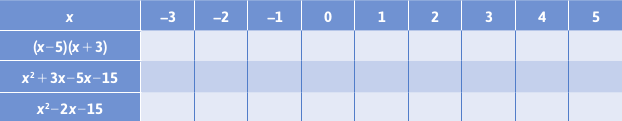
\includegraphics[width=0.8\textwidth]{tabla01.png}
              \captionof{figure}{Modelo geométrico de la situación.}
              \label{tab:table01}
          \end{figure}

          \begin{enumerate}
              \item ¿Cómo son los valores de las tres expresiones? ¿Qué pueden concluir sobre ellas?
              \item ¿Cómo pueden saber que un producto de expresiones algebraicas es equivalente a una ecuación de segundo grado?
          \end{enumerate}


    \item Se tienen dos expresiones algebraicas: $(x - 1)(x - 6) = 0$ y $x^2 - 7x + 6 = 0$.

          \begin{enumerate}
              \item ¿Cuál es una ecuación cuadrática? ¿Por qué?
              \item ¿Cuántas soluciones tiene la ecuación (x - 1)(x - 6) = 0? Explica.
              \item ¿Cuántas soluciones tendrá la ecuación x$^2 - 7x + 6 = 0$? ¿Por qué?
              \item ¿Cuántas soluciones tendrá una ecuación cuadrática?
                    Analicen los siguientes casos:
                    \[(x)(x) = 1 \text{\quad y \quad} x^2 = 1\]
                    \[x(x - 1) = 0 \text{\quad y \quad}x^2 - x = 0\]
                    \[(x - 1)(x - 2) = 0 \text{\quad y \quad} x^2 - 3x + 2 = 0\]
                    \[(x - 1)(x - 2) + 1 = 0 \text{\quad y \quad} x^2 - 3x + 3 = 0\]
                    Comprueben primero que cada par de ecuaciones es equivalente. Pueden probar por ensayo y error para
                    encontrar las soluciones.\\
          \end{enumerate}
\end{enumerate}

\begin{boxK}
    \begin{center}\textbf{Cierre}\end{center}

    \begin{minipage}[t]{0.2\textwidth}
        \begin{figure}[H]
            \centering
            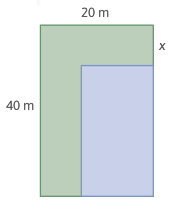
\includegraphics[width=\linewidth]{s7l1_cierre.png}
            \captionof{figure}{Modelo geométrico de la situación.}
            \label{fig:s7l1_cierre}
        \end{figure}
    \end{minipage}\hfill
    \begin{minipage}[t]{0.8\textwidth}
        \begin{enumerate}
            \item Retoma la situación de la actividad de inicio y responde, completa o corrige
                  tus respuestas. ¿Qué pasaría con las soluciones de la ecuación si los 120 son
                  metros cuadrados?
                  Reflexiona acerca de los conocimientos o las habilidades que necesitabas al
                  inicio y que ahora has adquirido. Escribe en tu cuaderno una conclusión.
            \item Los desarrolladores de un fraccionamiento habían planeado que algunos
                  terrenos para construir las casas fueran de 20 por 40 metros, pero los
                  40 m
                  reducirán de tal manera que tengan 525 m$^2$ de área para ampliar los adadores, como se muestra en la figura \ref{fig:s7l1_cierre}.
                  \begin{enumerate}
                      \item ¿De cuánto será el ancho del camino?
                      \item ¿Cómo planteas la ecuación que permite resolver el problema?
                  \end{enumerate}
        \end{enumerate}
    \end{minipage}


\end{boxK}

\newpage

\subsection{Gr\'aficas de expresiones cuadráticas y soluciones de sus ecuaciones}
\begin{boxK}
    \begin{center}\textbf{Inicio}\end{center}
    \begin{enumerate}
        \item Lee la situación, observa la imagen y responde lo que se pide.
              La torre Eiffel tiene una altura de 324 m. Desde la parte superior se deja caer una pelota
              de golf. La gráfica que se muestra es la representación de la ecuación que describe este
              movimiento, sin considerar la resistencia del aire. \\
              \textbf{¿Cuánto tiempo tarda el objeto en llegar al suelo?}
              \begin{enumerate}
                  \item ¿Qué parte de la gráfica tiene sentido considerar?
                  \item ¿Qué altura corresponde al tiempo 0 s? ¿A qué tiempo corresponde la altura 0 m?
                  \item ¿Qué valor es la solución del problema? Explica.
                  \item ¿Qué significa en la situación el valor simétrico, es decir, de signo contrario, al que obtuviste en la pregunta anterior?
                  \item ¿Qué información es relevante para responder y cuál no?
                  \item Describe el procedimiento que realizaste para saber las respuestas.
              \end{enumerate}
        \item  Reúnanse en equipo. Comparen sus respuestas, argumenten. Corrijan si es necesario.
              Reflexionen sobre el uso de gráficas para describir y resolver ecuaciones.
              \begin{figure}[H]
                  \centering
                  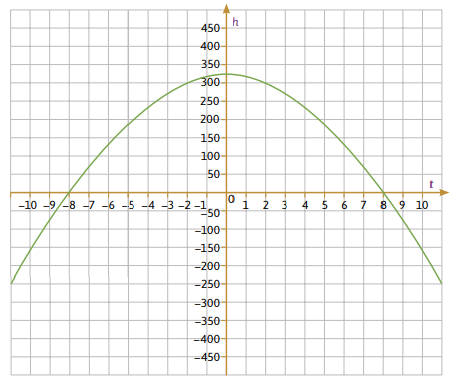
\includegraphics[width=0.65\textwidth]{parabole01.png}
                  \captionof{figure}{Modelo geométrico de la situación.}
                  \label{fig:parabole01}
              \end{figure}

    \end{enumerate}
\end{boxK}

\newpage

\subsubsection{Soluciones de ecuaciones cuadráticas con gráficas}

Analizaremos diversas gráficas de variaciones cuadráticas para determinar
la relación entre éstas y las soluciones de la ecuación asociada.

\begin{enumerate}
    \item Responde a los siguientes incisos.
          \begin{enumerate}

              \begin{minipage}[t]{0.3\textwidth}
                  \begin{figure}[H]
                      \centering
                      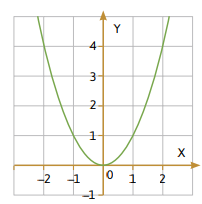
\includegraphics[width=\linewidth]{parabole02.png}
                      \captionof{figure}{Gráfica de $y = x^2$}
                      \label{fig:parabole02}
                  \end{figure}
              \end{minipage}\hfill
              \begin{minipage}[t]{0.6\textwidth}
                  \item Analicen la gráfica de $y = x^2$ (figura \ref{fig:parabole02}).
                  \begin{enumerate}
                      \item Localiza los puntos en los que la gráfica interseca al eje X. ¿Cuál
                            es el valor de $x$ en esos puntos?
                      \item Sustituye esos valores en la ecuación $x^2= 0$. ¿Qué observas?
                      \item Elije otros dos puntos que estén sobre la gráfica. ¿Cuál es el valor de $x$ en esos puntos?
                      \item Sustituyan esos nuevos valores en la ecuación $x^2= 0$. ¿Qué observas?
                  \end{enumerate}
              \end{minipage}

              \begin{minipage}[t]{0.6\textwidth}
                  \item Analiza la gráfica de $y = x - 1$ (figura \ref{fig:parabole03}) y responde.
                  \begin{enumerate}
                      \item Localiza los puntos en los que la gráfica interseca al eje X. ¿Cuál es el valor de $x$ en esos puntos?
                      \item Elije otros dos puntos que estén sobre la gráfica. ¿Cuál es el valor de $x$ en esos puntos?
                      \item Sustituye esos nuevos valores en la ecuación $x^2 - 1 = 0$. ¿Qué observas?
                      \item ¿Qué puedes decir acerca de las soluciones de la ecuación $x^2 - 1 = 0$?
                  \end{enumerate}
              \end{minipage}\hfill
              \begin{minipage}[t]{0.3\textwidth}
                  \begin{figure}[H]
                      \centering
                      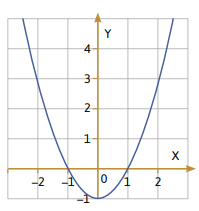
\includegraphics[width=\linewidth]{parabole03.png}
                      \captionof{figure}{Gráfica de $y = x^2 - 1$}
                      \label{fig:parabole03}
                  \end{figure}
              \end{minipage}

              \begin{minipage}[t]{0.3\textwidth}
                  \begin{figure}[H]
                      \centering
                      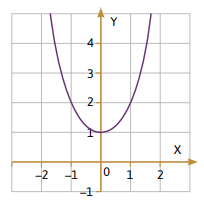
\includegraphics[width=\linewidth]{parabole04.png}
                      \captionof{figure}{Gráfica de $y = x^2 + 1$.}
                      \label{fig:parabole04}
                  \end{figure}
              \end{minipage}\hfill
              \begin{minipage}[t]{0.6\textwidth}
                  \item Analicen la gráfica de $y = x^2 + 1$  (figura \ref{fig:parabole04}).
                  \begin{enumerate}
                      \item Localiza los puntos en los que la gráfica interseca al eje X. ¿Cuál
                            es el valor de $x$ en esos puntos?
                      \item Elije otros dos puntos que estén sobre la gráfica. ¿Cuál es el valor de $x$ en esos puntos?
                      \item Sustituye esos nuevos valores en la ecuación $y = x^2 + 1$. ¿Qué observas?
                      \item ¿Qué puedes decir acerca de las soluciones de la ecuación $x^2 + 1 = 0$?
                  \end{enumerate}
              \end{minipage}
              ¿Qué semejanzas y diferencias observan entre las tres expresiones?
              ¿Y entre sus gráficas? Con base en las gráficas anteriores, ¿cuántas soluciones pue-
              de tener una ecuación cuadrática? ¿Cómo pueden determinar las soluciones?
          \end{enumerate}

          % \newpage

    \item Responde a los siguientes incisos.
          \begin{enumerate}

              \begin{minipage}[t]{0.3\textwidth}
                  \begin{figure}[H]
                      \centering
                      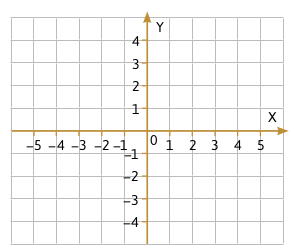
\includegraphics[width=\linewidth]{xyplane.png}
                      \captionof{figure}{}
                      \label{fig:xyplane}
                  \end{figure}
              \end{minipage}\hfill
              \begin{minipage}[t]{0.6\textwidth}
                  \item Considera la expresión $\frac{1}{2}x^2 + x$. Completa la tabla \ref{tab:table02} para
                  obtener algunos valores y con base en éstos realiza la gráfica en la figura \ref{fig:xyplane}.
                  Aproxima a un decimal.
                  \begin{figure}[H]
                      \centering
                      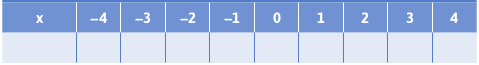
\includegraphics[width=0.9\linewidth]{tabla02.png}
                      \captionof{table}{}
                      \label{tab:table02}
                  \end{figure}
                  Con base en la gráfica, ¿cuántas soluciones tiene la ecuación $\frac{1}{2}x^2 + x= 0$? ¿Cuáles son?
              \end{minipage}

              \begin{minipage}[t]{0.6\textwidth}
                  \item Considera la expresión $\frac{1}{2}x^2 - x$. Completa la tabla \ref{tab:table03} para
                  obtener algunos valores y con base en éstos realiza la gráfica en la figura \ref{fig:xyplane2}.
                  Aproxima a un decimal.
                  \begin{figure}[H]
                      \centering
                      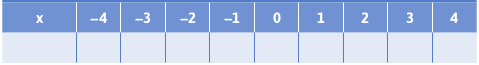
\includegraphics[width=0.9\linewidth]{tabla02.png}
                      \captionof{table}{}
                      \label{tab:table03}
                  \end{figure}
                  Con base en la gráfica, ¿cuántas soluciones tiene la ecuación $\frac{1}{2}x^2 - x= 0$? ¿Cuáles son?
              \end{minipage}\hfill
              \begin{minipage}[t]{0.3\textwidth}
                  \begin{figure}[H]
                      \centering
                      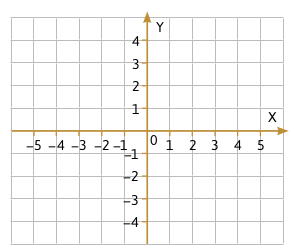
\includegraphics[width=\linewidth]{xyplane.png}
                      \captionof{figure}{}
                      \label{fig:xyplane2}
                  \end{figure}
              \end{minipage}

              \begin{minipage}[t]{0.3\textwidth}
                  \begin{figure}[H]
                      \centering
                      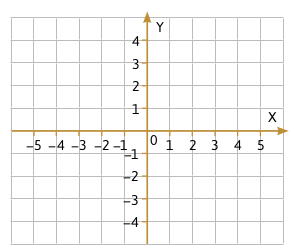
\includegraphics[width=\linewidth]{xyplane.png}
                      \captionof{figure}{}
                      \label{fig:xyplane3}
                  \end{figure}
              \end{minipage}\hfill
              \begin{minipage}[t]{0.6\textwidth}
                  \item Considera la expresión $-\frac{1}{2}x^2 + x$. Completa la tabla \ref{tab:table04} para
                  obtener algunos valores y con base en éstos realiza la gráfica en la figura \ref{fig:xyplane3}.
                  Aproxima a un decimal.
                  \begin{figure}[H]
                      \centering
                      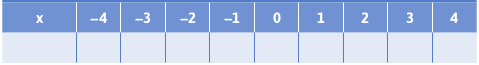
\includegraphics[width=0.9\linewidth]{tabla02.png}
                      \captionof{table}{}
                      \label{tab:table04}
                  \end{figure}
                  Con base en la gráfica, ¿cuántas soluciones tiene la ecuación $-\frac{1}{2}x^2 + x= 0$? ¿Cuáles son?
              \end{minipage}

              \begin{minipage}[t]{0.6\textwidth}
                  \item Considera la expresión $-\frac{1}{2}x^2 - x$. Completa la tabla \ref{tab:table05} para
                  obtener algunos valores y con base en éstos realiza la gráfica en la figura \ref{fig:xyplane4}.
                  Aproxima a un decimal.
                  \begin{figure}[H]
                      \centering
                      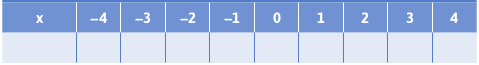
\includegraphics[width=0.9\linewidth]{tabla02.png}
                      \captionof{table}{}
                      \label{tab:table05}
                  \end{figure}
                  Con base en la gráfica, ¿cuántas soluciones tiene la ecuación $-\frac{1}{2}x^2 - x= 0$? ¿Cuáles son?
              \end{minipage}\hfill
              \begin{minipage}[t]{0.3\textwidth}
                  \begin{figure}[H]
                      \centering
                      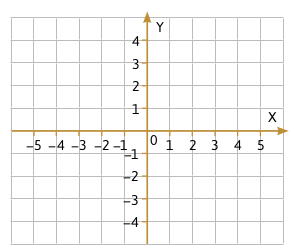
\includegraphics[width=\linewidth]{xyplane.png}
                      \captionof{figure}{}
                      \label{fig:xyplane4}
                  \end{figure}
              \end{minipage}
          \end{enumerate}
          ¿Qué semejanzas y diferencias observan entre las tres expresiones?
          ¿Y entre sus gráficas? Con base en las gráficas anteriores, ¿cuántas soluciones pue-
          de tener una ecuación cuadrática? ¿Cómo pueden determinar las soluciones?

          \begin{boxH}
              Las gráficas de expresiones cuadráticas pueden ser \emph{abiertas hacia arriba o hacia
                  abajo}. También pueden estar a la izquierda o derecha del origen.
              \begin{figure}[H]
                  \centering
                  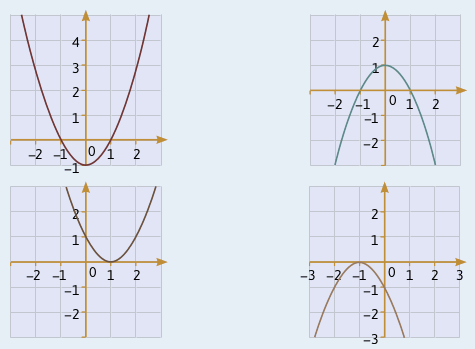
\includegraphics[width=\linewidth]{paraboles.png}
                  \captionof{figure}{}
                  \label{fig:paraboles}
              \end{figure}
          \end{boxH}

          \newpage

    \item Analiza las gráficas de la figura \ref{fig:paraboles2.6}. Determina el número
          de soluciones que tiene la ecuación en cada caso y escríbanlas.

          \begin{figure}[H]
              \centering
              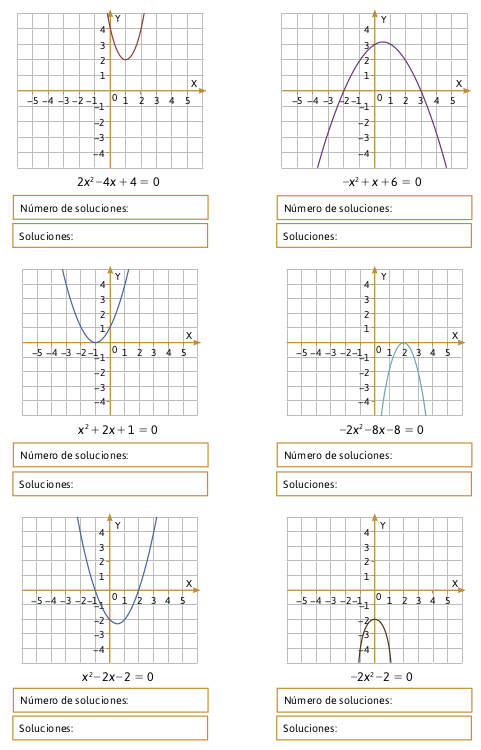
\includegraphics[width=0.8\linewidth]{paraboles2.6.png}
              \captionof{figure}{Gráficas de expresiones cuadráticas.}
              \label{fig:paraboles2.6}
          \end{figure}

          Con base en la gráfica de una expresión cuadrática de
          la forma $ax^2 + bx + c$, ¿cómo determinan el número de soluciones de la
          ecuación $ax^2 + bx + c = 0$? ¿Cómo determinan las soluciones? Escriban
          una conclusión en su cuaderno.
\end{enumerate}

\begin{boxK}
    \begin{center}\textbf{Cierre}\end{center}

    \begin{enumerate}
        \item Retoma la situación de la actividad de inicio y responde, completa o corrige
              tus respuestas. Si la gráfica abriera hacia arriba, ¿qué representaría?
              Reflexiona acerca de los conocimientos o las habilidades que necesitabas al
              inicio y que ahora has adquirido. Escribe en tu cuaderno una conclusión.
        \item María ha graficado la expresión $y = x^2-8x + 15$ para resolver las siguientes
              ecuaciones:
              \begin{itemize}
                  \item $x^2-8x + 15 = -2$
                  \item $x^2-8x + 15 = -1$
                  \item $x^2-8x + 15 = 0$
                  \item $x^2-8x + 15 = 1$
                  \item $x^2-8x + 15 = 2$
              \end{itemize}
              \begin{enumerate}
                  \item Traza las rectas que son paralelas al eje X y que pasan por $y = -2$, $y = -1$, $y = 0$, $y = 1$ y $y = 2$.
                  \item Localiza los puntos en los que interseca cada recta a la gráfica.
                  \item ¿Cuáles son los valores de $x$ de esos puntos?
                  \item Evalúa los valores obtenidos de cada intersección en su ecuación correspondiente. Por ejemplo, los valores obtenidos para la variable $x$ de la intersección de la recta que pasa por $y = 2$ y la gráfica en la ecuación $x^2 - 8x + 15 = 2$. ¿Qué observas?
                  \item ¿María puede resolver las ecuaciones con ayuda de la gráfica sin hacer operaciones? Explica.
              \end{enumerate}
    \end{enumerate}

    \begin{figure}[H]
        \centering
        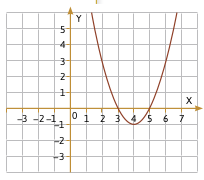
\includegraphics[width=0.4\linewidth]{s7l2_cierre.png}
        \captionof{figure}{}
        \label{fig:s7l2_cierre}
    \end{figure}
\end{boxK}

\begin{boxF}
    En un partido de campeonato, un futbolista patea el balón. Con
    base en la toma de una cámara, la computadora del centro de
    transmisión traza la trayectoria del balón y calcula la ecuación
    que la describe: $y = - \frac{1}{8}x^2 + 58 x + 74$ . Según la gráfica el futbolista
    está en el punto $x = -2$. ¿Hasta qué punto llegará la pelota?
    \begin{enumerate}
        \item ¿Qué parte de la gráfica tiene sentido según el problema?
        \item ¿Cuáles son las soluciones de la ecuación $-\frac{1}{8}x^2 + 58 x + 74 = 0$?
        \item ¿Qué significado tienen las soluciones dentro del problema?
        \item Si un jugador del equipo contrario que mida 1.80 m de altura
              se ubicara en $x = 0$, ¿taparía el disparo? Explica.
    \end{enumerate}

    \begin{figure}[H]
        \centering
        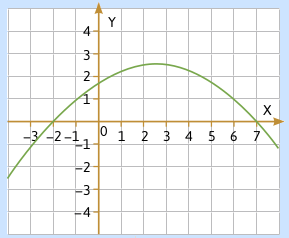
\includegraphics[width=0.4\linewidth]{futbolista.png}
        \captionof{figure}{Gráfica de la ecuación que representa la trayectoria del balón.}
        \label{fig:futbolista}
    \end{figure}
\end{boxF}

\newpage \thispagestyle{plain}
\section{Resolución de ecuaciones cuadráticas}

\boxabstract{Resuelve problemas mediante la formulación y la solución algebraica de ecuaciones cuadráticas.}
\subsection{Procedimientos para la resolución de ecuaciones cuadráticas}

\begin{boxK}
    \begin{center}\textbf{Inicio}\end{center}
    \begin{enumerate}
        \item Observa la figura \ref{fig:camino} y responde lo que se pide.
              Un jardín rectangular mide 50 m por 40 m. Se quiere construir un camino de ancho
              constante alrededor del jardín como se muestra en la figura. ¿Qué tan ancho deberá
              ser el camino si debe cubrir un área de 784 m$^2$ ?
              \begin{enumerate}
                  \item Escribe una ecuación que permita obtener el área del camino.
                  \item ¿Cuánto mide el ancho del camino? ¿Cuánta área verde quedará?
                  \item Realiza la gráfica que describe la expresión algebraica obtenida.
                  \item ¿Qué información es relevante para responder y cuál no?
                  \item Describe el procedimiento que realizaste para saber las respuestas.
              \end{enumerate}
        \item Reúnanse en equipo. Reflexionen sobre los procedimientos de solución
              de una ecuación cuadrática. Argumenten. Corrijan si es necesario.
              \begin{figure}[H]
                  \centering
                  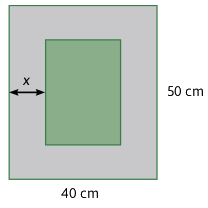
\includegraphics[width=0.4\textwidth]{camino.png}
                  \captionof{figure}{Modelo geométrico de la situación.}
                  \label{fig:camino}
              \end{figure}
    \end{enumerate}
\end{boxK}

\newpage

\subsubsection{Producto de factores lineales}
Responde a los siguientes incisos.
\begin{enumerate}
    \item Considera las ecuaciones $x(x - 9) = 0$ y $x^2 - 9x = 0$.
          \begin{enumerate}
              \item Considera la ecuación $(x)(x) - (9)(x) = 0$ y compárala con $x(x - 9) = 0$. ¿Qué observas? ¿Son equivalentes? Explica.
              \item Efectúa los productos en $(x)(x) - (9)(x) = 0$. ¿Qué expresión obtienes?
              \item ¿Las ecuaciones $x(x - 9) = 0$ y $x^2 - 9x = 0$ son equivalentes? ¿Por qué?
          \end{enumerate}
    \item Considera las ecuaciones $(x + 1)(x - 1) = 0$ y $x^2 - 1 = 0$.
          \begin{enumerate}
              \item Considera la ecuación $(x + 1)(x) + (x + 1)(-1) = 0$ y compárala con
                    $(x + 1)(x - 1) = 0$. ¿Qué observas? ¿Son equivalentes? Explica.
              \item Efectúa los productos en $(x + 1)(x) + (x + 1)(-1) = 0$. ¿Qué expresión obtienes?
              \item ¿Las ecuaciones $(x + 1)(x - 1) = 0$ y $x^2 - 1 = 0$ son equivalentes? ¿Por qué?
          \end{enumerate}

          ¿Cuál es el resultado de efectuar siguientes productos?:
          \[x(x + a)=\]
          \[x(x - a)=\]
          \[(x + a)(x + b)=\]
          \[(x + a)(x - b)=\]
          Supongan que $a$ y $b$ son enteros, fracciones o decimales. Observen con cuidado el manejo de
          los signos al multiplicar.

          \begin{boxH}
              Un \textbf{producto de factores lineales} tiene la forma general de
              \[(ax + b)(cx + d) = acx^2 + adx + bcx + bd = acx^2 + (ad + bc)x + bd\]
          \end{boxH}

          \subsubsection{La factorización para resolver ecuaciones cuadráticas}

          Desarrollaremos la relación que existe entre una ecuación cuadrática escrita como
          producto de expresiones lineales y las soluciones de la ecuación.

    \item Considera las ecuaciones $3x + 2 = 0$ y $x - 4 = 0$.
          \begin{enumerate}
              \item ¿Cuáles son las soluciones de $3x + 2 = 0$ y de $x - 4 = 0$?
              \item Ahora considera la ecuación $(3x + 2)(x - 4) = 0$. ¿Cómo puedes encontrar su solución? ¿Cuál es?
              \item ¿Hay alguna relación entre las soluciones de $3x + 2 = 0$ y $x - 4 = 0$ y las de $(3x + 2)(x - 4) = 0$? Explica.
              \item Efectúa el producto en la ecuación $(3x + 2)(x - 4) = 0$. ¿Qué ecuación obtienes?
              \item ¿Cuáles son las soluciones de la ecuación que obtuviste? ¿Por qué?
          \end{enumerate}

          \newpage

    \item Analiza la ecuación $(x - 1.2) (x + 3.3) = 0$.
          \begin{enumerate}
              \item Efectúen el producto. ¿Qué ecuación obtienen?
              \item ¿Cuáles son las raíces de la ecuación que obtuvieron?
              \item Compara tus respuestas y procedimientos. Si hay diferencias, argumenta. Corrijan si es necesario. Comenten: ¿cómo se relacio-
                    nan las soluciones de una ecuación en la que hay un producto de expresiones li-
                    neales y las de su equivalente ecuación cuadrática?
          \end{enumerate}

          \begin{boxH}
              \textbf{Factorizar} una ecuación cuadrática significa escribirla como el producto de dos
              términos algebraicos lineales. La nueva ecuación es equivalente a la primera y las
              soluciones se obtienen de resolver dos ecuaciones lineales.
              \begin{align*}
                  x^2 + 7x - 18  & = 0 \Rightarrow \\
                  (x + 9)(x - 2) & = 0
              \end{align*}
              y las soluciones a ambas ecuaciones son $x = - 9$ y $x = 2$.
          \end{boxH}

    \item Completa la tabla \ref{tab:table2.6}.

          \begin{figure}[H]
              \centering
              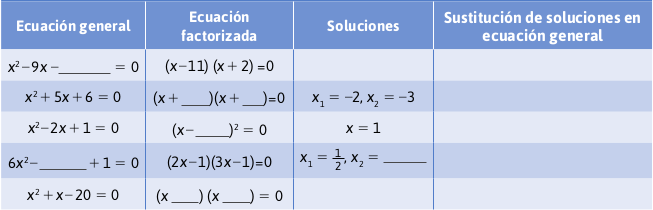
\includegraphics[width=0.9\textwidth]{table2.6.png}
              \captionof{table}{}
              \label{tab:table2.6}
          \end{figure}

          \subsubsection{Técnicas de factorización de ecuaciones cuadráticas}
          Desarrollaremos técnicas sencillas para factorizar ecuaciones cuadráticas.

    \item Desarrollen la ecuación $(x + 8)(x - 3) = 0$. Exprésenla como $ax^2 + bx + c = 0$.
          \begin{enumerate}
              \item ¿Cuál es el valor del coeficiente de $x^2$ ?
              \item ¿Cómo pueden obtener el coeficiente de $x$ con las raíces de $(x + 8)(x - 3) = 0$?
              \item ¿Cómo pueden obtener el término independiente con las raíces de $(x + 8)(x - 3) = 0$?
          \end{enumerate}

    \item Desarrolla la ecuación $(x + r)(x + s) = 0$. Exprésala en la forma $x^2 + bx + c = 0$.
          Consideren que $r$ y $s$ son números enteros, fraccionarios o decimales.
          \begin{enumerate}
              \item ¿Cuál es el valor del coeficiente de $x^2$ ?
              \item ¿Cómo pueden obtener el coeficiente de $x$ con las raíces de $(x + r)(x + s) = 0$?
              \item ¿Cómo pueden obtener el término independiente con las raíces de $(x + r)(x + s) = 0$?
          \end{enumerate}
    \item  Consideren la ecuación $x^2 + 9x + 18 = 0$.
          \begin{enumerate}
              \item ¿Cuáles son los coeficientes de $x^2$ y $x$? ¿Y el término independiente?
              \item Encuentren dos números tales que la suma de ellos sea igual al coeficiente de $x$ y el producto sea igual al término independiente.
              \item Con los números que determinaron, ¿pueden escribir la ecuación $x^2 + 9x + 18 = 0$ como un producto de dos factores lineales? ¿Cómo?
              \item ¿Cómo comprueban que la ecuación $x + 9x + 18 = 0$ y la que escribieron son equivalentes? Háganlo.
          \end{enumerate}

          ¿Cómo factorizan una ecuación cuadrática? ¿Cómo pueden validar su factorización? ¿Cómo pueden
          factorizar ecuaciones del tipo $ax^2 + c = 0$ y $ax^2 + bx = 0$? Propongan varios ejemplos
          y factorícenlos en el pizarrón. Despejen cualquier duda de sus compañeros. Escriban una conclusión en su cuaderno.

          \begin{boxH}
              La \textbf{factorización de la ecuación de segundo grado} $x^2 + bx + c = 0$ es una expresión
              de la forma $(x + r) (x + s) = 0$ donde las raíces son $-r$ y $-s$. Por ejemplo, la factoriza-
              ción de $x^2 - x - 2 = 0$ es $(x + 1) (x - 2) = 0$, cuyas raíces de ambas son $- 1$ y $2$.
              $r + s = -b$ y $r s = c$, es decir, que la suma de las raíces es el inverso aditivo del
              coeficiente de $x$ y el producto de las raíces es el término independiente de la ecuación cuadrática.
          \end{boxH}

    \item Completa la tabla \ref{tab:table2.7}.

          \begin{figure}[H]
              \centering
              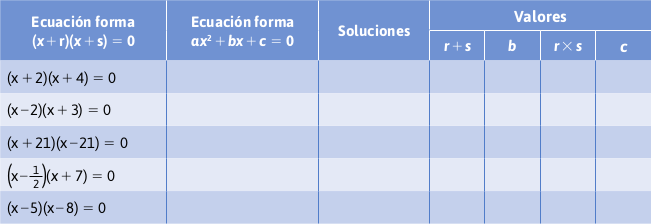
\includegraphics[width=0.9\textwidth]{table2.7.png}
              \captionof{table}{}
              \label{tab:table2.7}
          \end{figure}

    \item Completa la tabla \ref{tab:table2.8}.

          \begin{figure}[H]
              \centering
              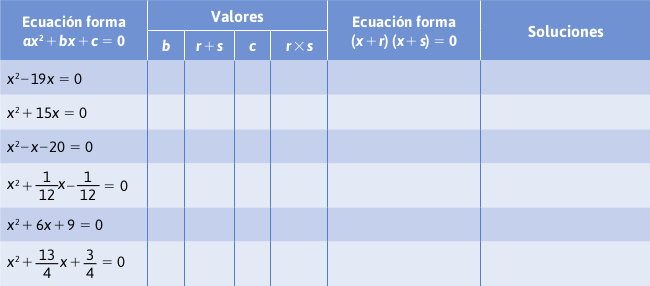
\includegraphics[width=0.9\textwidth]{table2.8.png}
              \captionof{table}{}
              \label{tab:table2.8}
          \end{figure}

    \item Analiza las ecuaciones $2x^2 + 3x - 2 = 0$ y $x^2 + 3 x - 1 = 0$.
          \begin{enumerate}
              \item ¿Observas alguna semejanza entre ambas? ¿Cuál?
              \item ¿Cuáles son las soluciones a la ecuación $x^2 + 3 x - 1 = 0$? Verifica tu respuesta.
              \item Las soluciones que encontraste, ¿son solución de $2x^2 + 3x - 2 = 0$? Explica
              \item ¿Las ecuaciones $2x^2 + 3x - 2 = 0$ y $x^2 + 3 x - 1 = 0$ son equivalentes? ¿Por qué?
          \end{enumerate}
          ¿Cómo dividen una ecuación $ax^2 + bx + c = 0$ entre $a$? ¿Siempre pueden dividir una ecuación
          $ax^2 + bx + c = 0$ entre $a$? ¿Cómo tiene que ser $a$? Consideren que $a$ es un número
          entero, fracción o decimal. Escriban una conclusión en su cuaderno.

    \item Completa la tabla \ref{tab:table2.9}.

          \begin{figure}[H]
              \centering
              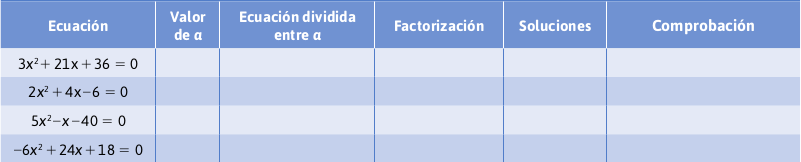
\includegraphics[width=\textwidth]{table2.9.png}
              \captionof{table}{}
              \label{tab:table2.9}
          \end{figure}

          \begin{enumerate}
              \item Expliquen cómo encontrar las raíces de una ecuación del tipo $ax^2 + bx + c = 0$.
              \item Comenten acerca del procedimiento para encontrar las raíces de $ax^2 + bx + c = 0$. Escriban una conclusión en su cuaderno.
          \end{enumerate}

          \begin{boxH}
              Una \textbf{ecuación cuadrática general} del tipo $ax^2 + bx + c = 0$, con $a$, $b$, $c$ números en-
              teros, fraccionarios o decimales y $a \neq 0$, es equivalente a la ecuación $x^2 + \frac{b}{a} x + \frac{c}{a} = 0$,
              la cual se puede factorizar buscando números cuya suma sea igual a $-\frac{b}{a}$ y cuyo
              producto sea igual a $\frac{c}{a}$.
          \end{boxH}

          \subsubsection{Problemas de factorización de ecuaciones cuadráticas}

    \item Escribe la ecuación cuadrática que tenga las raíces indicadas.
          \begin{enumerate}
              \item -1 y 3.
              \item 0 y -17.
              \item -8 y 8.
              \item 11 y 12.
          \end{enumerate}

    \item Resuelve las ecuaciones.
          \begin{enumerate}
              \item $x^2 -  x  - 20 = 0$.
              \item $x^2 + 9x  - 36 = 0$.
              \item $x^2 + 10x + 21 = 0$.
              \item $x^2 + 4x  - 32 = 0$.
          \end{enumerate}

          \begin{minipage}[t]{0.35\textwidth}
              \begin{figure}[H]
                  \centering
                  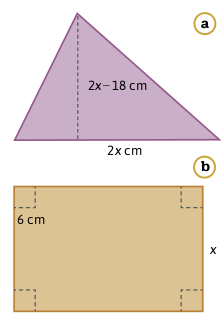
\includegraphics[width=\linewidth]{figuras2.7.png}
                  \captionof{figure}{(a) Triángulo, (b) Pieza rectangular para armar una caja.}
                  \label{fig:figuras2.7}
              \end{figure}
          \end{minipage}\hfill
          \begin{minipage}[t]{0.5\textwidth}
              \item El área de un rectángulo es 28 cm$^2$. Tiene 3 cm más de largo que de ancho. ¿Cuáles son sus dimensiones?
              \item Un terreno rectangular tiene área de 750 m$^2$. Se coloca una cerca alrededor de los 110 m de perímetro. Calcula las dimensiones del terreno.
              \item Un rectángulo tiene el ancho más corto que el largo por 3 cm. El área de la figura es de 51 cm$^2$. ¿Qué medidas tiene?
              \item El triángulo de la figura \ref{fig:figuras2.7}a tiene área igual a 52 cm$^2$, encuentra las medidas de su base y de su altura.
              \item Una pieza rectangular como la de la figura \ref{fig:figuras2.7}b es 4 cm más larga que ancha. Con ella se construye una caja de 840 cm$^3$ cortando un cuadrado
              en cada esquina y doblando los bordes. Escribe las medidas de la altura y el volumen de la caja, así como los lados de la pieza rectangular.

          \end{minipage}

\end{enumerate}


\begin{boxK}
    \begin{center}\textbf{Cierre}\end{center}

    \begin{enumerate}
        \item Retoma la situación de la actividad de inicio y responde, completa o corrige
              tus respuestas. ¿Qué pasaría con el ancho del camino y el área verde si el
              valor de $x$ se redujera a la mitad?
              Reflexiona acerca de los conocimientos o las habilidades que necesitabas al
              inicio y que ahora has adquirido. Escribe en tu cuaderno una conclusión.
        \item Dentro de 15 años, la edad de Elena en ese entonces multiplicada por 6 será
              un tercio del cuadrado de la edad actual. ¿Cuántos años tiene Elena hoy?

              \begin{enumerate}
                  \item Escribe una ecuación que describa el problema.
                  \item ¿Hay más de una solución? Explica por qué y escríbelas, si es el caso.
              \end{enumerate}
    \end{enumerate}
\end{boxK}

\newpage

\subsection{Fórmula general de la ecuación de segundo grado}

\begin{boxK}
    \begin{center}\textbf{Inicio}\end{center}
    \begin{enumerate}
        \item Lee la situación, observa la imagen de la figura \ref{fig:ayb} y responde lo que se pide.
              \begin{figure}[H]
                  \centering
                  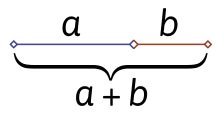
\includegraphics[width=0.4\textwidth]{ayb.png}
                  \captionof{figure}{}
                  \label{fig:ayb}
              \end{figure}
              \begin{boxF}
                  Dos números a y b, distintos de 0, están en proporción áurea si se cumple que:
                  \[\dfrac{a + b}{a}=\dfrac{a}{b}\]
                  de donde, después de hacer algunos cálculos, se obtiene la expresión
                  \[ \left(\dfrac{a}{b}\right)^2-\left(\dfrac{a}{b}\right)-1=0\]
                  en la que $\frac{b}{a}$ es la razón áurea. ¿Cuál es este valor?
              \end{boxF}
              \begin{enumerate}
                  \item Si consideramos que $\frac{b}{a}$ se puede representar por otra variable, por ejemplo $x$, entonces, ¿cómo se escribe la ecuación?
                  \item Los valores $\dfrac{1+\sqrt{5}}{2}$ y $\dfrac{1-\sqrt{5}}{2}$, ¿son soluciones de la ecuación?
                  \item Factoriza la ecuación.
                  \item ¿Cómo piensas que se podría resolver esta ecuación sin factorizar?
                  \item ¿Qué información es relevante para responder y cuál no?
                  \item Describe el procedimiento que realizaste para saber las respuestas.
              \end{enumerate}
    \end{enumerate}
\end{boxK}

\subsubsection{Fórmula general para resolver ecuaciones cuadráticas}
La fórmula general sirve para resolver ecuaciones de segundo grado de todo tipo.

\begin{enumerate}
    \item Considera la ecuación $3x^2 - 7x - 6 = 0$.
          \begin{enumerate}
              \item Encuentra las soluciones de la ecuación. Verifica que lo sean.
              \item Compara la ecuación $3x^2 - 7x - 6 = 0$ con la forma general de una cuadrática $ax ^2 + bx + c = 0$. ¿Cuáles son los valores de $a$, $b$ y $c$?
              \item Sustituye los valores anteriores en las siguientes expresiones. Realiza las operaciones necesarias para resolver y escribe las soluciones obtenidas.

                    $ x_1= \dfrac{-b+\sqrt{b^2-4ac}}{2a} = $ \\[3ex]
                    $ x_2= \dfrac{-b-\sqrt{b^2-4ac}}{2a} = $
              \item Compara tus resultados con los del inciso a). ¿Qué observas?
          \end{enumerate}

    \item Consideren la ecuación $3x^2 + 25x - 28 = 0$.
          \begin{enumerate}
              \item Comparen la ecuación con la forma general de una ecuación cuadrática. Anoten
                    los valores de:

                    $a =$ \rule{15mm}{0.2mm}\\
                    $b =$ \rule{15mm}{0.2mm}\\
                    $c =$ \rule{15mm}{0.2mm}\\

              \item Sustituye los valores de $a$, $b$ y $c$ en las expresiones siguientes. Realiza las operaciones necesarias para resolver y escribe las soluciones obtenidas.

                    $ x_1= \dfrac{-b+\sqrt{b^2-4ac}}{2a} = $ \\[3ex]
                    $ x_2= \dfrac{-b-\sqrt{b^2-4ac}}{2a} = $

              \item  Escriban los valores obtenidos de $x_1$ y $x_2$ con una aproximación de dos decimales.
              \item ¿Cómo pueden verificar que $x_1$ y $x_2$ son soluciones de la ecuación $3x^2 + 25x - 28 = 0$? ¿Qué observan al hacer esta verificación?
          \end{enumerate}

          \begin{boxH}
              Las soluciones $x_1$ y $x_2$ de una ecuación cuadrática de la forma $ax^2 + bx + c = 0$ están dadas por las expresiones
              \[ x_1= \dfrac{-b+\sqrt{b^2-4ac}}{2a} \text{ y }  x_2= \dfrac{-b-\sqrt{b^2-4ac}}{2a}\]
              que se pueden escribir en una sola expresión:
              \[x= \dfrac{-b\pm\sqrt{b^2-4ac}}{2a}\]
              en la que el signo $\pm$ (más menos) indica que para obtener una raíz se suma - b y
              $\sqrt{b^2 - 4ac}$ y para obtener la otra se resta $- b$ y $\sqrt{b^2 - 4ac}$. Esta última expresión se
              conoce como \textbf{fórmula general} para resolver ecuaciones de segundo grado.
          \end{boxH}

          \newpage

    \item Hagan los cálculos en su cuaderno y anoten sus resultados aquí, para obtener las soluciones para cada ecuación e la siguiente tabla.

          \begin{figure}[H]
              \centering
              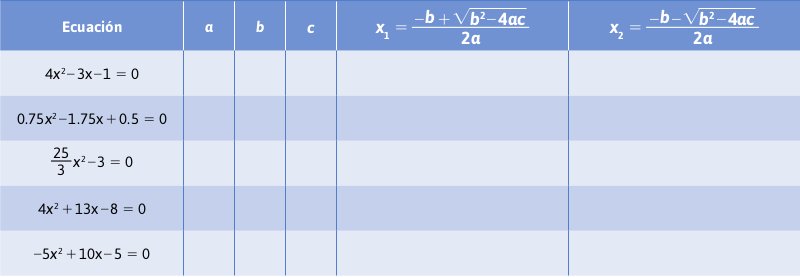
\includegraphics[width=\textwidth]{table2.10.png}
              \captionof{table}{}
              \label{tab:table2.10}
          \end{figure}

    \item Resuelvan las ecuaciones con el método que cada uno prefiera:

          \begin{enumerate}
              \item $3x^2  - 2x - 4 = 0$.
              \item $2x^2 - 5x + 2 = 0$.
              \item $x^2 - x - 6 = 0$.
              \item $x^2 + 2x + 1 = 0$.
              \item $9x^2 - 42x + 40 = 0$.
              \item $0.4^2 - 2x - 3 = 0$.
              \item $\frac{3}{4}x^2 + 6x - 3 = 0$.
              \item $x^2 - 2x - 3 = 0$.
          \end{enumerate}

          En su cuaderno, expliquen en qué casos usaron la fórmula general y por qué. ¿Usaron otros métodos de solución? ¿Cuáles? ¿Por qué?

    \item Se quiere construir una ventana en la que su perímetro y área
          están determinados de antemano (figura 2.8). ¿Cuáles debe ser sus dimensiones?
          \begin{enumerate}
              \item ¿De qué manera expresas algebraicamente el largo del rectángulo? ¿Y su ancho? Explica.
              \item Escribe una ecuación cuadrática que describa el problema.
              \item Escribe las soluciones de la ecuación.
              \item ¿Cuáles son las medidas de la ventana?
          \end{enumerate}

          \newpage

          \subsubsection{Discriminante}
          El discriminante permite determinar si una ecuación cuadrática tiene ninguna, una o
          dos soluciones.

    \item Responde a los siguientes incisos.
          \begin{enumerate}
              \item Consideren la ecuación $x^2 - 6x + 5 = 0$. Realicen lo que se pide. Hagan las operaciones en su cuaderno y anoten los resultados aquí.
                    \begin{itemize}
                        \item Ubiquen los valores de a, b y c correspondientes a la ecuación $x^2 - 6x + 5 = 0$ y obtengan sus soluciones.
                        \item ¿Cuál es el valor de la expresión $b^2 - 4ac$? ¿Se puede calcular $\sqrt{b^2 - 4ac}$? ¿Por qué?
                        \item ¿Observan alguna relación entre el valor de $b^2 - 4ac$ y el número de soluciones de la ecuación $x^2 - 6x + 5 = 0$? ¿Cuál?
                    \end{itemize}

              \item Consideren la ecuación $3x^2 + 24x + 48 = 0$. Hagan las operaciones en su cuaderno y anoten los resultados aquí.
                    \begin{itemize}
                        \item Ubiquen los valores de $a$, $b$ y $c$ correspondientes a la ecuación $3x^2 + 24x + 48 = 0$ y obtengan sus soluciones.
                        \item ¿Cuál es el valor de la expresión $b^2 - 4ac$? ¿Se puede calcular $\sqrt{b^2 - 4ac}$? ¿Por qué?
                        \item ¿Observan alguna relación entre el valor de $b^2 - 4ac$ y el número de soluciones de la ecuación $3x^2 + 24x + 48 = 0$? ¿Cuál?
                    \end{itemize}

              \item Consideren la ecuación $\frac{1}{2}x^2 + 5x + 15 = 0$. Hagan las operaciones en su cuaderno y anoten los resultados aquí.
                    \begin{itemize}
                        \item Ubiquen los valores de $a$, $b$ y $c$ correspondientes a la ecuación $\frac{1}{2}x^2 + 5x + 15 = 0$ y obtengan sus soluciones.
                        \item ¿Cuál es el valor de la expresión $b^2 - 4ac$? ¿Se puede calcular $\sqrt{b^2 - 4ac}$? ¿Por qué?
                        \item ¿Observan alguna relación entre el valor de $b^2 - 4ac$ y el número de soluciones de la ecuación $\frac{1}{2}x^2 + 5x + 15 = 0$? ¿Cuál?
                    \end{itemize}
          \end{enumerate}

    \item Completa la tabla \ref{tab:table2.11}.

          \begin{figure}[H]
              \centering
              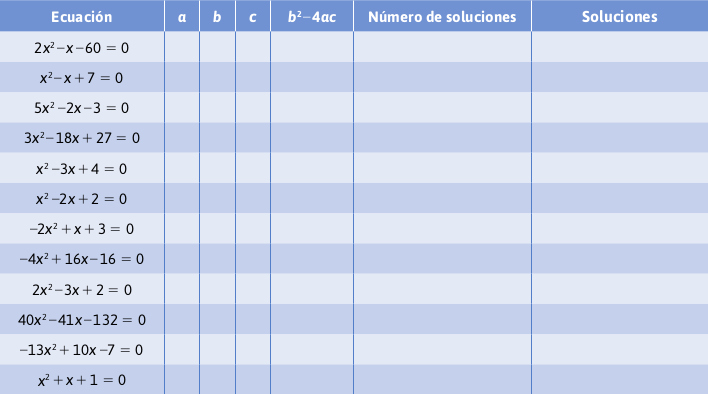
\includegraphics[width=\textwidth]{table2.11.png}
              \captionof{table}{}
              \label{tab:table2.11}
          \end{figure}

          \begin{enumerate}
              \item Si $b^2 - 4ac = 0$, ¿cuántas soluciones tiene la ecuación cuadrática? ¿Por qué?
              \item Sí $b^2 - 4ac > 0$, ¿cuántas soluciones tiene la ecuación cuadrática? ¿Por qué?
              \item Si $b^2 - 4ac < 0$, ¿cuántas soluciones tiene la ecuación cuadrática? ¿Por qué?
              \item ¿Cuál es la importancia de calcular $b^2 - 4ac$? Escriban una conclusión en su cuaderno.
          \end{enumerate}

          \begin{boxH}
              La ecuación cuadrática $ax^2 + bx + c = 0$ tiene:
              \begin{itemize}
                  \item Dos soluciones si $b^2 - 4ac > 0$ y las raíces son

                        \[x_1 = \frac{-b + \sqrt{b^2 - 4ac}}{2a} \text{ y } x_2 = \frac{-b - \sqrt{b^2 - 4ac}}{2a}\]

                  \item Una solución si $b^2 - 4ac = 0$ y la raíz es

                        \[x = \frac{-b}{2a}\].

                  \item Ninguna solución real si $b^2 - 4ac < 0$.
              \end{itemize}

          \end{boxH}

          \begin{boxH}
              A la expresión \textbf{$b^2 - 4ac$} se le conoce como el \textbf{discriminante} de la ecuación
              cuadrática.
          \end{boxH}
\end{enumerate}

\newpage

\subsubsection{Problemas con ecuaciones de segundo grado}

\begin{enumerate}
    \item Contesta.
          \begin{enumerate}
              \item ¿Cuántas raíces tiene la ecuación $9x^2 - 2x + 4 = 0$?
              \item Escribe una ecuación que tenga soluciones $x_1 = 0.3$ y $x_2 = 0.7$.
              \item Anota una ecuación que tenga una sola solución $x = -3$.
          \end{enumerate}

    \item Si al producto de un número natural por su consecutivo le restamos 31, obtenemos
          el quíntuple de la suma de ambos. ¿De qué números se trata?

    \item Un proyectil es lanzado verticalmente y la expresión $h(t) = 512t - 16t^2$ describe la
          altura $h$ de su posición después de $t$ segundos.
          \begin{enumerate}
              \item ¿Qué altura alcanza después de 6 segundos?
              \item ¿El proyectil alcanza la altura de 3,520 m? Si es así, ¿en qué tiempo la alcanza?
              \item ¿En qué momento alcanza la altura de 5,500 m?
              \item ¿En cuánto tiempo regresará a la tierra? Explica.

          \end{enumerate}

    \item Un terreno rectangular tiene dimensiones de 8 m por 24 m. Si el ancho y el largo
          aumentan en una misma cantidad fija, el área aumenta 144 m$^2$. ¿Cuántos metros
          aumentan el largo y el ancho del terreno?
          \begin{enumerate}
              \item ¿Cuántos metros aumentaron las dimensiones?
              \item ¿Cuáles son las nuevas medidas del largo y el ancho?
          \end{enumerate}

    \item Si $P$ pesos se invierten a dos años con un interés anual $x$; a ese interés, la inversión
          crecerá a otra cantidad $A$, también en pesos, mediante la fórmula $A = P(1 + x)^2$.
          ¿A qué tasa de interés $x$, una cantidad inicial de \$1,000.00 crecerá a \$1,200.00 en los dos años?

    \item Dos automóviles viajan a velocidades uniformes sobre la misma ruta cubriendo una distancia de 180 km. Uno va 5 km más despacio que otro y tarda 30 min más en hacer el recorrido. ¿A qué velocidad va cada automóvil?

    \item En un concurso de matemáticas, se planteó un problema sobre una ecuación de segundo grado. Un estudiante lo resuelve pero se equivoca en el término independiente (c) y obtiene como soluciones: 9 y 3. Otro estudiante se equivoca en el coeficiente del término de primer grado (b) y obtiene como soluciones: -7 y -5. ¿Cuál fue la ecuación planteada del problema?


\end{enumerate}

\begin{boxK}
    \begin{center}\textbf{Cierre}\end{center}

    \begin{enumerate}
        \item Retoma la situación de la actividad de inicio y responde, completa o corrige tus respuestas. ¿Qué pasaría si en la razón, se cambia $a - b$ en lugar de $a + b$?
              ¿Es más fácil resolver la ecuación? ¿Por qué?
              Reflexiona acerca de los conocimientos o las habilidades que necesitabas al inicio y que ahora has adquirido. Escribe en tu cuaderno una conclusión.
        \item El sistema romano de proporciones arquitectónicas se basa
              en el llamado número de plata. Un rectángulo cuya relación entre los lados sea igual al número de plata se denomina
              rectángulo plateado. Resuelve la ecuación $x^2 - 2x - 1 = 0$ para conocer su valor. ¿Cuántas soluciones tiene? ¿Qué solución es la que tiene sentido? Explica.
    \end{enumerate}

    \begin{figure}[H]
        \centering
        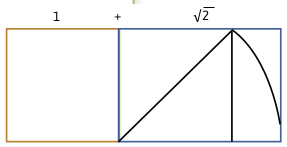
\includegraphics[width=0.6\textwidth]{plata.png}
        \captionof{figure}{Rect\'angulo de plata.}
        \label{fig:plata}
    \end{figure}

\end{boxK}

\begin{boxF}
    Los matemáticos de la antigüedad buscaron cómo definir la belleza y
    establecieron que una figura que tenga proporción áurea nos resultará
    preciosa y hermos a. Denominaron a esta proporción el número de oro
    $\Phi$ (fi). Para calcularlo se basaron en una definición: una forma es bella
    cuando la proporción entre el total y su parte mayor (razón extrema) es
    igual a la proporción entre su parte mayor y su parte menor (razón media).
    Éste es el concepto de belleza que tomó \textbf{Leonardo da Vinci (1452-
        1519)} en su famosa obra \emph{El hombre de Vitruvio}. Con base en la figura,
    calcula el valor del número de oro.

    \[ \frac{\Phi+1}{\Phi} = \frac{\Phi}{1} \]

    \begin{figure}[H]
        \centering
        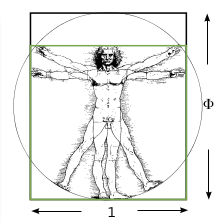
\includegraphics[width=0.4\textwidth]{hombre.png}
        \captionof{figure}{Bosquejo de \emph{El hombre de Vitruvio} por Leonardo da Vinci.}
        \label{fig:hombre}
    \end{figure}

\end{boxF}

\newpage \thispagestyle{plain}
\section{Relación entre variación y ecuación cuadrática}
\boxabstract{Resuelve problemas mediante la formulación y la solución algebraica de ecuaciones cuadráticas.}
\subsection{Variación cuadrática y ecuación asociada}

\begin{boxK}
    \begin{center}\textbf{Inicio}\end{center}

\end{boxK}

\begin{boxK}
    \begin{center}\textbf{Cierre}\end{center}

\end{boxK}

\subsection{Modelación de situaciones de variación cuadrática}

\begin{boxK}
    \begin{center}\textbf{Inicio}\end{center}

\end{boxK}

\begin{boxK}
    \begin{center}\textbf{Cierre}\end{center}

\end{boxK}

\newpage \thispagestyle{plain}
\section{Características de la variación}

\boxabstract{Analiza y compara diversos tipos de variación a partir de sus representaciones tabular, gráfica y algebraica, que resultan de modelar situaciones y fenómenos de la Física y de otros contextos.}
\subsection{Distintos tipos de variación}

\begin{boxK}
    \begin{center}\textbf{Inicio}\end{center}

\end{boxK}

\begin{boxK}
    \begin{center}\textbf{Cierre}\end{center}

\end{boxK}

\subsection{Dependencia y razón de cambio}

\begin{boxK}
    \begin{center}\textbf{Inicio}\end{center}

\end{boxK}

\begin{boxK}
    \begin{center}\textbf{Cierre}\end{center}

\end{boxK}

\newpage \thispagestyle{plain}
\section{Análisis de la variación cuadrática}

\boxabstract{Analiza y compara diversos tipos de variación a partir de sus representaciones tabular, gráfica y algebraica, que resultan de modelar situaciones y fenómenos de la Física y de otros contextos.}

\subsection{Representación tabular de la variación cuadrática}

\begin{boxK}
    \begin{center}\textbf{Inicio}\end{center}

\end{boxK}

\begin{boxK}
    \begin{center}\textbf{Cierre}\end{center}

\end{boxK}

\subsection{Representación algebraica de la variación cuadrática}

\begin{boxK}
    \begin{center}\textbf{Inicio}\end{center}

\end{boxK}

\begin{boxK}
    \begin{center}\textbf{Cierre}\end{center}

\end{boxK}

\subsection{Representación gr\'afica de la variación cuadrática}

\begin{boxK}
    \begin{center}\textbf{Inicio}\end{center}

\end{boxK}

\begin{boxK}
    \begin{center}\textbf{Cierre}\end{center}

\end{boxK}

\subsection{Representación tabular, algebraica y gr\'afica de variaciones cuadráticas}

\begin{boxK}
    \begin{center}\textbf{Inicio}\end{center}

\end{boxK}

\begin{boxK}
    \begin{center}\textbf{Cierre}\end{center}

\end{boxK}

\newpage \thispagestyle{plain}
\section{Variaciones diversas}

\boxabstract{Analiza y compara diversos tipos de variación a partir de sus representaciones tabular, gráfica y algebraica, que resultan de modelar situaciones y fenómenos de la Física y de otros contextos.}

\subsection{Interpretación de gr\'aficas}

\begin{boxK}
    \begin{center}\textbf{Inicio}\end{center}

\end{boxK}

\begin{boxK}
    \begin{center}\textbf{Cierre}\end{center}

\end{boxK}

\subsection{Construcción de gr\'aficas a partir de tablas}

\begin{boxK}
    \begin{center}\textbf{Inicio}\end{center}

\end{boxK}

\begin{boxK}
    \begin{center}\textbf{Cierre}\end{center}

\end{boxK}

\subsection{Análisis de gr\'aficas de variaciones diversas}

\begin{boxK}
    \begin{center}\textbf{Inicio}\end{center}

\end{boxK}

\begin{boxK}
    \begin{center}\textbf{Cierre}\end{center}

\end{boxK}

\newpage \thispagestyle{plain}
\section{Eventos mutuamente excluyentes}
\subsection{Eventos singulares y no singulares}
\subsection{Eventos mutuamente excluyentes}
\subsection{Unión de dos eventos}
\subsection{Regla de la suma de probabilidades}

%%% U3
\chapter{}

\newpage \thispagestyle{plain}
\section{Expresiones algebraicas de segundo grado}
\subsection{Áreas y expresiones de segundo grado}
\subsection{Operaciones algebraicas}
\subsection{Factorización de expresiones de segundo grado}

\newpage \thispagestyle{plain}
\section{Expresiones algebraicas de ecuaciones y funciones}
\subsection{Expresiones algebraicas de ecuaciones}
\subsection{Expresiones algebraicas de funciones}

\newpage \thispagestyle{plain}
\section{Teorema de Pitágoras}
\subsection{Triángulos rectángulos y el teorema de Pitágoras}
\subsection{El teorema de Pitágoras}
\subsection{Aplicaciones del teorema de Pitágoras}

\newpage \thispagestyle{plain}
\section{Razones trigonométricas (seno, coseno y tangente)}
\subsection{Razones trigonométricas básicas}
\subsection{Razones trigonométricas de 30$^{\circ}$, 45$^{\circ}$ y 60$^{\circ}$}

\newpage \thispagestyle{plain}
\section{Resolución de triángulos rectángulos}
\subsection{Seno, coseno y tangente de ángulos agudos}
\subsection{Aplicaciones de razones trigonométricas}





\end{document}






